\section{Results}

\subsection{Introduction}
In this section we present data gathered from our experiments on the ARM
Cortex-A9.

We distinguish between single-cycle instructions and multi-cycle instructions
because they behave differently in and around the execution pipeline.
Instructions consuming only one cycle are fairly easy to reason about as there
is no need to normalize energy consumption with respect to the cycle count (i.e.
time). However, it is important to also recognize CPU capabilities such as dual
issuing that we have on our processor: All single-cycle ALU instructions execute
pairwise in parallel (one in each ALU), giving a peak performance of two
instructions per CPU cycle. On the other hand, multi-cycle instructions needs to
be carefully considered. Typically, multi-cycle instructions divide work which
can be done only in a subset of the available CPUs (e.g. one) over several
cycles, lowering the average current draw. They consume less energy per
timestep, but also do less useful work.

For all these reasons, we partition the measured data in two datasets; one for
single-cycle instructions and one for multi-cycle instructions.

\subsection{Single-Cycle Instructions}
On our target CPU, most of \todo{how many} the tested instructions falls into
this category. The per-instruction energy consumption measured in Ampere can be
seen in figure \ref{fig:singlecycle}.

\begin{figure}
    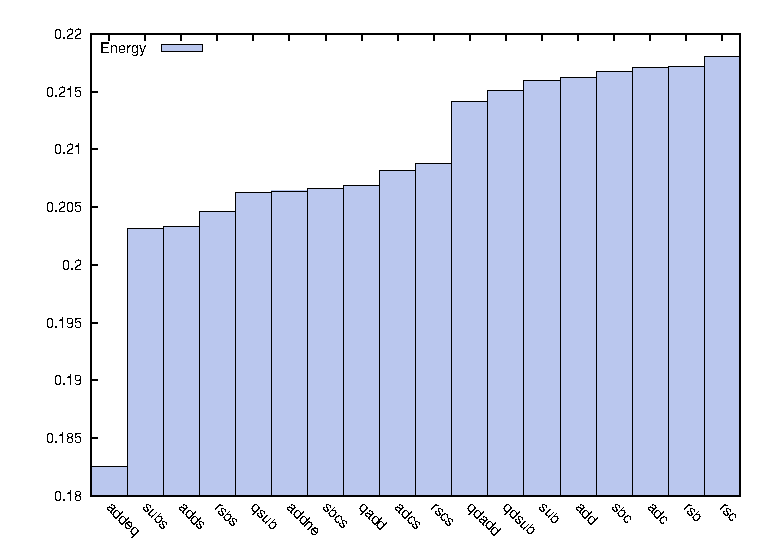
\includegraphics[width=\textwidth/2]{figures/single-cycle}
    \caption{Single Cycle energy consumption}
    \label{fig:singlecycle}
\end{figure}

\subsection{Multi-Cycle Instructions}
\todo[inline]{This section is mostly an outline}
Some instructions use variable amount of time. This section will contain
information about how we normalize and compare energy consumption of
these instructions. It will be difficult to compare single cycle instructions
to the multi cylce ones, as the single cycle instructions is often the ones
utilizing more than one ALU at a time. Also, the multi-cycle ones will most
likly pipeline up very differently than the single cycle ones. We will try to
draw a conclusion about the results, but it is important to note the differences
in the execution path of these two categeories.
